\documentclass[14pt]{beamer}
\usetheme{EastLansing}
\usecolortheme{spruce}

\usepackage{xcolor}
\usepackage{listings}
\usepackage{courier}
\usepackage{graphicx}
\usepackage{amsmath}
\usepackage{algorithm2e}
\usepackage{multicol}

% https://tex.stackexchange.com/questions/42619/x-mark-to-match-checkmark
\usepackage{pifont}% http://ctan.org/pkg/pifont

%% https://stackoverflow.com/questions/1435837/how-to-remove-footers-of-latex-beamer-templates
%%gets rid of bottom navigation bars
%\setbeamertemplate{footline}[page number]
%
%gets rid of navigation symbols
\setbeamertemplate{navigation symbols}{}


\usefonttheme[onlymath]{serif}

\definecolor{mGreen}{rgb}{0,0.6,0}
\definecolor{mGray}{rgb}{0.5,0.5,0.5}
\definecolor{mPurple}{rgb}{0.8,0,0.82}
\definecolor{backgroundColour}{rgb}{0.95,0.95,0.92}
\definecolor{lightBlue}{rgb}{0.1, 0.1, 0.8}

\newcommand\red[1]{{\color{red} #1}}
\newcommand\green[1]{{\color{green} #1}}
\newcommand\blue[1]{{\color{blue} #1}}

\newcommand{\cmark}{\ding{51}}%
\newcommand{\xmark}{\ding{55}}%

\lstdefinestyle{CStyle}{
    backgroundcolor=\color{backgroundColour},   
    commentstyle=\color{mGreen},
    keywordstyle=\color{magenta},
    numberstyle=\tiny\color{mGray},
    stringstyle=\color{mPurple},
    basicstyle=\footnotesize,
    breakatwhitespace=false,         
    breaklines=true,                 
    captionpos=b,                    
    keepspaces=true,                 
    numbers=left,                    
    numbersep=5pt,                  
    showspaces=false,                
    showstringspaces=false,
    showtabs=false,                  
    tabsize=2,
    language=C
}
\lstdefinestyle{pseudo}{
        basicstyle=\ttfamily\footnotesize,
        keywordstyle=\color{lightBlue},
        morekeywords={BEGIN,END,IF,ELSE,ENDIF,ELSEIF,PRINT,WHILE,RETURN,ENDWHILE,DO,FOR,TO,IN,ENDFOR,BREAK,INPUT},
        morecomment=[l]{//},
        commentstyle=\color{mGreen}
}

\lstset{basicstyle=\footnotesize\ttfamily,breaklines=true}
\lstset{framextopmargin=50pt,tabsize=2}

\title{ENGG1003 - Monday Week 4}
\subtitle{Iteration again: \texttt{for} vs.~\texttt{while} loops, \\ debugging strategies \& random numbers}
\author{Steve Weller}
\institute{University of Newcastle}
%\date{\today}
\date{15 March, 2021}

% following is a bit of a hack, but forces page numbers (technically: frame numbers) to run 1,2,3,... 
% with titlepage counting as frame 1

\addtocounter{framenumber}{1}
\titlepage

\begin{document}
\framebreak

%==============================================================

\begin{frame}[fragile]

\frametitle{Lecture overview}
\begin{enumerate}
	\item iteration again (again): \texttt{for} vs.~\texttt{while} loops \red{\S3.3.3}

	\item[]
	
	\item debugging strategies
	
	\item[]
	
	\item random numbers in Python \red{\S2.4}

\end{enumerate}

\end{frame}

%==============================================================

\begin{frame}[fragile]

\frametitle{$1)$ iteration again: \texttt{for} vs.~\texttt{while} loops}

\begin{itemize}
	\item side-by-side comparison for print-1-to-10
	\item similarities and differences
	\item when to use each
\end{itemize}

\end{frame}

%==============================================================

\begin{frame}[fragile]

\frametitle{}

\begin{itemize}
	\item xxx
\end{itemize}

\end{frame}

%==============================================================

\begin{frame}[fragile]

\frametitle{Example: Finding the maximum height}

\begin{itemize}
	\item \S3.3.3
	\item new program instead finds the maximum height achieved by the ball
	\item will solve in two ways: for and while
\end{itemize}

\end{frame}

%==============================================================

\begin{frame}[fragile]

\frametitle{}

\begin{figure}[ht]
	\centering
	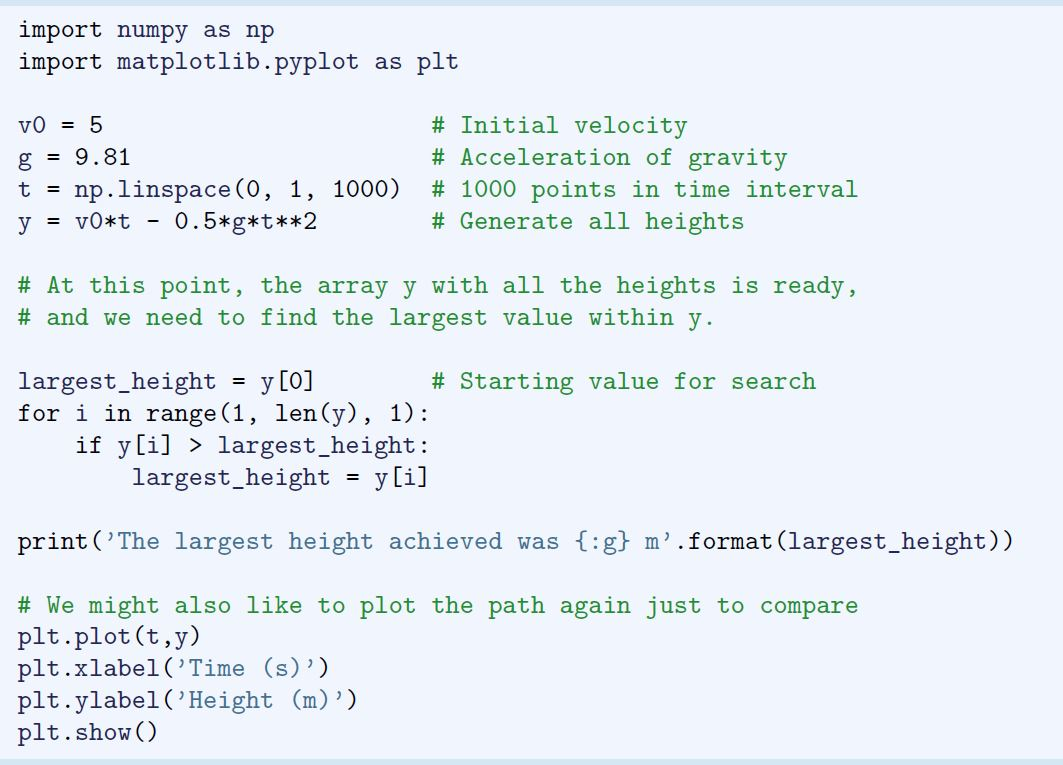
\includegraphics[width=\textwidth]{figures/LLp71a}
\end{figure}

\end{frame}

%==============================================================

\begin{frame}[fragile]

\frametitle{Focus on code to find max using for}

\begin{itemize}
	\item describe strategy in words
	\item live demo
\end{itemize}

% We focus our attention on the new thing here, the search performed by the for
%loop. The value in y[0] is used as a starting value for largest_height. The very
%first check then, tests whether y[1] is larger than this height. If so, y[1] is stored
%as the largest height. The for loop then updates i to 2, and continues to check
%y[2], and so on. Each time we find a larger number, we store it. When finished,
%largest_height will contain the largest number from the array y.

\begin{figure}[ht]
	\centering
	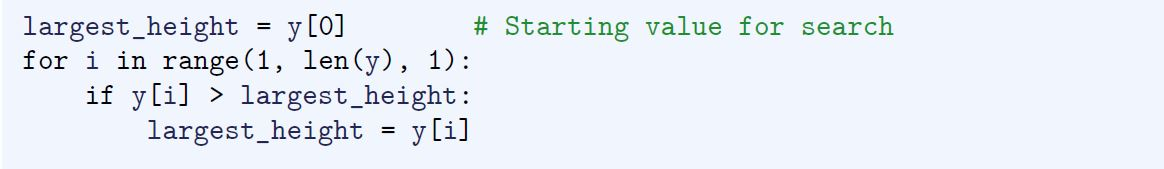
\includegraphics[width=\textwidth]{figures/LLp71b}
	
\includegraphics[width=\textwidth]{figures/LLp71c}
\end{figure}

\end{frame}

%==============================================================

\begin{frame}[fragile]

\frametitle{Focus on code to find max using while}

\begin{itemize}
	\item describe strategy in words
	\item live demo
\end{itemize}

%The observant reader has already seen the similarity of finding the maximum
%height and finding the time of flight, as we addressed previously in Sect. 3.2.1.
%In fact, we could alternatively have solved the maximum height problem here by
%utilizing that y[i+1] > y[i] as the ball moves towards the top. Doing this, our
%search loop could have been written
%i = 0
%while y[i+1] > y[i]:
%i = i + 1
%When the condition y[i+1] > y[i] becomes False, we could report y[i+1] as
%our approximation of the maximum height, for example.

\begin{figure}[ht]
	\centering
	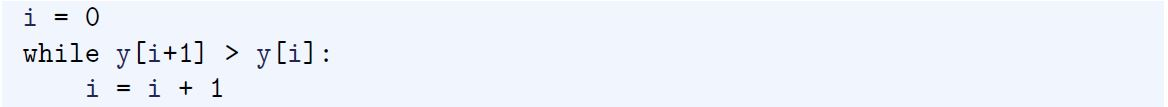
\includegraphics[width=\textwidth]{figures/LLp71d}
\end{figure}

\end{frame}

%==============================================================

\begin{frame}[fragile]

\frametitle{$2)$ debugging strategies}

\begin{enumerate}
	\item running code by hand
	\item don't guess, print!
	\item take baby steps
	\item use comments to hide debug code
\end{enumerate}

\end{frame}

%==============================================================

\begin{frame}[fragile]

\frametitle{running code by hand}

\begin{itemize}
	\item Work through your code line-by-line, with a piece of paper and a pen
	\item Use paper/notes-app before you run code, so that you know what you want program to calculate on each line before you run code
	\item Second-best: use notes app on iPad or similar---idea is to \emph{think before computing}
	\item Check that every line of code, with every use of an array index (hint) matches what you expect
	\item Near enough isn't good enough here. Think like a computer: work systematically through each line of code. Is it doing what you want it to do?
	\item It's easy (but often misleading) to look at code and think you know what it's doing. But is it really?
	\item mindset shift: rather than hoping or thinking it's OK, try and find the bug (might be more than one)
\end{itemize}

\end{frame}

%==============================================================

\begin{frame}[fragile]

\frametitle{don't guess, print!}

\begin{itemize}
	\item xxx
\end{itemize}

\end{frame}

%==============================================================

\begin{frame}[fragile]

\frametitle{take baby steps}

\begin{itemize}
	\item xxx
\end{itemize}

\end{frame}

%==============================================================

\begin{frame}[fragile]

\frametitle{use comments to hide debug code}

\begin{itemize}
	\item but don't delete it
\end{itemize}

\end{frame}

%==============================================================

\begin{frame}[fragile]

\frametitle{$3)$ random numbers in Python}

\begin{itemize}
	\item Python provides ability to produce (apparently) random numbers
	\item referred to as \red{\emph{pseudo-random numbers}}
	\item these numbers are not truly random, but produced in a predictable way once a \red{\emph{seed}} has been set
	\item the seed is a number which depends on the current time
%	\begin{itemize}
%		\item restartin your computer in between the two runs, get a new
%	\end{itemize}
		
\end{itemize}

%. 

%\begin{itemize}
%	\item drawing \textbf{one} random number at a time
%	\item drawing \textbf{many} random numbers at a time
%\end{itemize}

\end{frame}

%==============================================================

\begin{frame}[fragile]

\frametitle{Drawing \textbf{one} random number at a time}

\begin{itemize}
	\item LL p54
	\item \verb+throw_2_dice.py+
	\item live demo
	\item function randint is available from the imported module random, which is part of the standard Python library
	\item randint(a,b) returns a pseudo-random \emph{integer} in the range $[a,b]$ where $a \leq b$
\end{itemize}

\end{frame}

%==============================================================

\begin{frame}[fragile]

\frametitle{Fixing the seed}

\begin{itemize}
	\item When debugging programs that involve pseudo-random number generation, it is a great advantage to \red{\emph{fix the seed}}
	\item ensures that the very same sequence of numbers will be generated each time the code is run
	\item simply means that you pick the seed yourself and tell Python what that seed should be
	\item example: random.seed(10)
	\item live demo of  \verb+throw_2_dice.py+
\end{itemize}

\end{frame}

%==============================================================

\begin{frame}[fragile]

\frametitle{Two useful functions: random and uniform}

\begin{itemize}
	\item both of these functions return a floating point number from an interval where each number has equal probability of being drawn
	\item confusing: random function in random module
	\item random, the interval is always [0, 1) (i.e. 0 is included, but 1 is not)
	\item uniform requires the programmer to specify the interval [a, b] (where both a and b are included)
	\item text doesn't mention Gaussian (normal) random numbers
\end{itemize}

\end{frame}

%==============================================================

\begin{frame}[fragile]

\frametitle{Live demo: random and uniform}

\begin{itemize}
	\item LLp55 screengrab
	\item live demo
	\item a word about In[] and Out[]
\end{itemize}

\begin{figure}[ht]
	\centering
	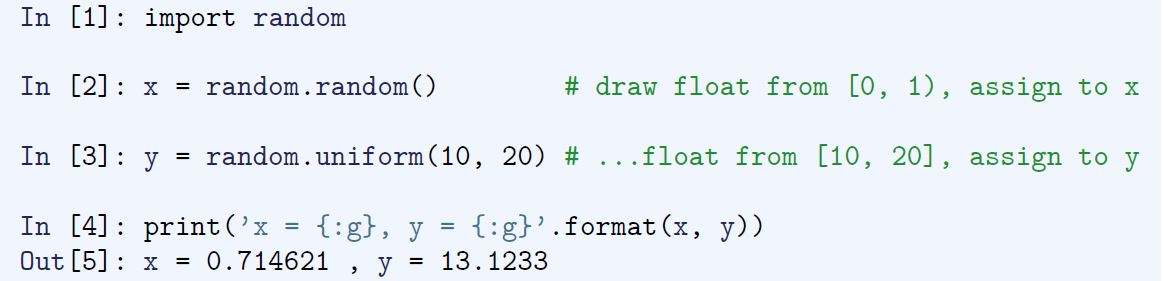
\includegraphics[width=\textwidth]{figures/LLp55a}
\end{figure}

\end{frame}

%==============================================================

\begin{frame}[fragile]

\frametitle{Drawing \textbf{many} random numbers at a time}

\begin{itemize}
	\item three PRN generators so far: one at a time
	\item could use in a loop, call once each time
	\item much better: vectorization (have seen before)
	\item need another module called random
	\begin{itemize}
		\item this one inside numpy library
	\end{itemize}
\end{itemize}

\end{frame}

%==============================================================

\begin{frame}[fragile]

\frametitle{Live demo: random numbers from numpy library}

\begin{itemize}
	\item LLp55b screen grab
	\item live demo
	\item np.random.randint
	\begin{itemize}
		\item np library, random module, randint function
	\end{itemize}
\end{itemize}

\begin{figure}[ht]
	\centering
	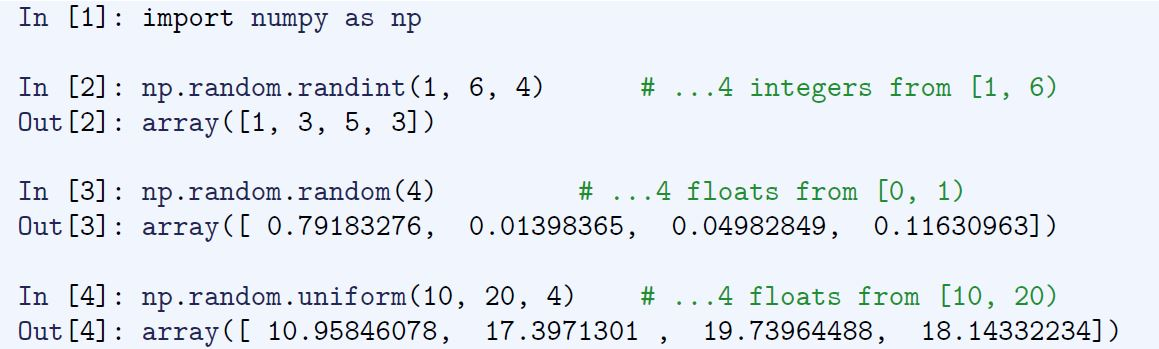
\includegraphics[width=\textwidth]{figures/LLp55b}
\end{figure}

\end{frame}

%==============================================================

\begin{frame}[fragile]

\frametitle{}

\begin{itemize}
	\item live demo
	\item numpy allows the seed to be set. For example, setting the seed to 10 (as above), could be done by
np.random.seed(10)
\end{itemize}

\end{frame}

%==============================================================

\begin{frame}[fragile]

\frametitle{Lecture summary}
\begin{itemize}
	\item Iteration again
	\begin{itemize}
		\item for vs while
	\end{itemize}

	\item[]
	
	\item debugging strategies
		\begin{itemize}
			\item blah
			\item blah
			\item blah
		\end{itemize}

	\item[]
	
	\item random numbers
		\begin{itemize}
			\item random module: randint, random and uniform
			\item random module in numpy library: randint, random and uniform
		\end{itemize}
		
\end{itemize}

\end{frame}

\end{document}